\documentclass[a4paper, 12pt]{article}

\input{/home/nick/latex-preambles/xelatex.tex}

\setmainfont{Minion Pro}

\newcommand{\imagesPath}{.}

\title{
	\textbf{Εργαστήριο Δικτύων Υπολογιστών} \\~\\
	Εργαστηριακή Άσκηση 4 \\ 
	Εισαγωγή στη δρομολόγηση
}
\author{}
\date{}

\begin{document}
\maketitle
\begin{center}
	\begin{tabular}{|l|l|}
		\hline
		\textbf{Ονοματεπώνυμο:} Νικόλαος Παγώνας, el18175  & \textbf{Όνομα PC:} nick-ubuntu \\
		\hline
		\textbf{Ομάδα:} 1 (Τρίτη 10:45) & \textbf{Ημερομηνία Εξέτασης:} Τρίτη 29/03/2022 \\
		\hline
	\end{tabular}
\end{center}

\section*{Άσκηση 1 (προετοιμασία): Διευθύνσεις IP}

	\subsection*{1.1}
		Ο αριθμός δικτύου δεν είναι παρά ένα μέρος της διεύθυνσης IP. Συνολικά, η διεύθυνση IP αποτελείται από τον αριθμό δικτύου και τον αριθμό host.

	\subsection*{1.2}
		Ο αριθμός δικτύου της διεύθυνσης \verb|192.220.147.2/22| είναι \verb|192.220.144| (προκύπτει από την σύζευξη της διεύθυνσης IP με τη μάσκα υποδικτύου).

	\subsection*{1.3}
		Για $100$ συσκευές χρειαζόμαστε $7$ bits ($2^7 = 128$). Αυτό σημαίνει ότι μένουν για τα διαφορετικά υποδίκτυα $32 - 22 - 7 = 3$ bits, άρα μπορούν να δημιουργηθούν $2^3 = 8$ υποδίκτυα.

	\subsection*{1.4}
		Η κλάση C παρέχει 254 διευθύνσεις για συσκευές.

	\subsection*{1.5}
		\begin{enumerate}[label=\alph*.]
			\item Όχι. 
			\item Ναι, εμπίπτει στην περιοχή \verb|10.0.0.0/8|.
			\item Όχι.
			\item Όχι.
			\item Nαι, εμπίπτει στην περιοχή \verb|192.168.0.0/16|.
		\end{enumerate}

	\subsection*{1.6}
		Ο δρομολογητής καταλαβαίνει ότι μπορεί να στείλει απευθείας πακέτα σε κάποια συσκευή μέσω των διεπαφών του, αν δει ότι η συσκευή βρίσκεται στο ίδιο υποδίκτυο με αυτόν (δηλαδή στο ίδιο υποδίκτυο με κάποια από τις διεπαφές του). Ο έλεγχος γίνεται εφαρμόζοντας την κατάλληλη μάσκα υποδικτύου κάθε φορά.

	\subsection*{1.7}
		Η διεύθυνση εκπομπής στο δίκτυο \verb|10.50.10.0/23| είναι η \verb|10.50.11.255/23|.

	\subsection*{1.8}
		Η κλάση της διεύθυνσης \verb|208.23.55.11| είναι C, επειδή τα πρώτα τρία bit είναι 110.

	\subsection*{1.9}
		Το πλήθος των διευθύνσεων που είναι διαθέσιμες για συσκευές στο δίκτυο \verb|147.102.0.0/17| είναι $2^{15}-2$, γιατί έχουμε $32-17=15$ bits για τον αριθμό host, και το $-2$ προκύπτει επειδή δεν μετράμε τη διεύθυνση δικτύου και τη διεύθυνση εκπομπής.

	\subsection*{1.10}
		Οι διευθύνσεις του ΕΜΠ ξεκινούν με $147 = 1001 \ 0011$, οπότε τα 2 πρώτα bit είναι $10$. Αυτό σημαίνει ότι ανήκουν στην κλάση B.

	\subsection*{1.11}
		\begin{itemize}
			\item Υποδίκτυο με 100 υπολογιστές: \verb|10.11.12.0/25|.
			\item Υποδίκτυο με 60 υπολογιστές: \verb|10.11.12.128/26|.
			\item Υποδίκτυο με 20 υπολογιστές: \verb|10.11.12.192/27|.
			\item Υποδίκτυο με 10 υπολογιστές: \verb|10.11.12.224/28|.
		\end{itemize}

	\subsection*{1.12}
		Ναι, υπάρχει χώρος για ένα ακόμη υποδίκτυο, το οποίο μπορεί να έχει μέχρι $2^4-2=14$ υπολογιστές. 

	\subsection*{1.13} 
		Μπορούμε να τις συντμήσουμε ομαδοποιώντας τις ως εξής: \\
		
		171.12.4.0/24, 171.12.5.0/24, 171.12.6.0/24, 171.12.7.0/24 $\rightarrow$ 171.12.4.0/22 \\
		
		171.12.8.0/24 $\rightarrow$ 171.12.8.0/24 (δεν μπορεί να γίνει κάποιου είδους σύντμηση)\\ 
		
		Να σημειωθεί ότι δεν μπορούμε να κάνουμε μία σύντμηση του τύπου 171.12.0.0/20 που θα συμπεριλάμβανε και τις 5 παραπάνω διευθύνσεις, διότι έτσι συμπεριλαμβάνουμε ένα υπερσύνολο των παραπάνω διευθύνσεων, οι οποίες δεν είναι δεδομένες.
		
\section*{Άσκηση 2: Ένα απλό δίκτυο}

	\subsection*{2.1}
		Ναι, χρησιμοποιήσαμε την επιλογή αυτή, ώστε οι εικονικές κάρτες δικτύου να έχουν μοναδικές φυσικές διευθύνσεις, όπως συμβαίνει και με τις κανονικές κάρτες δικτύου.

	\subsection*{2.2}
		Εκτελούμε ping από το PC1 στα PC2, PC3, PC4 και καταγράφουμε τα αποτελέσματα. \\
		
		Οι εντολές είναι: 
		
		\begin{verbatim}
			ping 192.168.1.2
			ping 192.168.1.18
			ping 192.168.1.29
		\end{verbatim}
		
		Και τα αποτελέσματα:
		
		\begin{itemize}
			\item PC1 $\rightarrow$ PC2: Επιτυχές.
			\item PC1 $\rightarrow$ PC3: Επιτυχές.
			\item PC1 $\rightarrow$ PC4: Δεν λαμβάνεται ποτέ απάντηση.
		\end{itemize}

	\subsection*{2.3}
		Εκτελούμε ping από το PC2 στα PC3, PC4 και καταγράφουμε τα αποτελέσματα. \\
		
		Οι εντολές είναι: 
		
		\begin{verbatim}
			ping 192.168.1.18
			ping 192.168.1.29
		\end{verbatim}
		
		Και τα αποτελέσματα:
		
		\begin{itemize}
			\item PC2 $\rightarrow$ PC3: No route to host.
			\item PC2 $\rightarrow$ PC4: No route to host.	
		\end{itemize}

	\subsection*{2.4}
		Εκτελούμε ping από το PC4 στα PC1, PC2, PC3 και καταγράφουμε τα αποτελέσματα. \\
		
		Οι εντολές είναι: 
		
		\begin{verbatim}
			ping 192.168.1.1
			ping 192.168.1.2
			ping 192.168.1.18
		\end{verbatim}
		
		Και τα αποτελέσματα:

		\begin{itemize}
			\item PC4 $\rightarrow$ PC1: No route to host.
			\item PC4 $\rightarrow$ PC2: No route to host.
			\item PC4 $\rightarrow$ PC3: Επιτυχές.
		\end{itemize}

	\subsection*{2.5}
		Εκτελούμε ping από το PC3 στα PC1, PC2 και καταγράφουμε τα αποτελέσματα. \\
		
		Οι εντολές είναι: 
		
		\begin{verbatim}
			ping 192.168.1.1
			ping 192.168.1.2
		\end{verbatim}
		
		Και τα αποτελέσματα:

		\begin{itemize}
			\item PC3 $\rightarrow$ PC1: Επιτυχές.
			\item PC3 $\rightarrow$ PC2: Δεν λαμβάνεται ποτέ απάντηση.		
		\end{itemize}

	\subsection*{2.6}
		Σε ορισμένα από τα προηγούμενα ping εμφανίζεται "No route to host" διότι ο αποστολέας, εφαρμόζοντας τη μάσκα υποδικτύου τόσο στη δική του διεύθυνση, όσο και στου παραλήπτη, διαπιστώνει ότι αποστολέας και παραλήπτης δεν βρίσκονται στο ίδιο υποδίκτυο, και άρα απαιτείται η παρουσία δρομολογητή για να φτάσουν τα πακέτα του ping στον προορισμό τους. Αφού δεν υπάρχει δρομολογητής, δεν υπάρχει και διαδρομή προς τον παραλήπτη, εξού και το μήνυμα "No route to host". \\
		
		Για παράδειγμα, όταν ο PC2 κάνει ping στο PC3, έχουμε:
		
		\begin{verbatim}
			PC2:
			192.168.1.2 & 255.255.255.240 = 192.168.1.0
			192.168.1.18 & 255.255.255.240 = 192.168.1.16
			192.168.1.0 != 192.168.1.16, so PC2 and PC3 are not in the same subnet.
		\end{verbatim}

	\subsection*{2.7}
		Σε ορισμένα από τα προηγούμενα ping δεν λαμβάνουμε απάντηση, διότι ο αποστολέας, εφαρμόζοντας τη μάσκα υποδικτύου του τόσο στη δική του διεύθυνση, όσο και στου παραλήπτη, θεωρεί πως βρίσκεται στο ίδιο υποδίκτυο με τον παραλήπτη, όμως αυτή τη φορά ο παραλήπτης, εφαρμόζοντας τη δική του μάσκα υποδικτύου, διαπιστώνει ότι δεν βρίσκεται στο ίδιο υποδίκτυο με τον αποστολέα. Αυτό έχει ως συνέπεια να στέλνει μεν ο αποστολέας τα πακέτα του ping προς τον παραλήπτη, όμως ο παραλήπτης δεν στέλνει ποτέ απάντηση.
		
		Για παράδειγμα, όταν ο PC1 κάνει ping στο PC4, έχουμε:
		
		\begin{verbatim}
			PC1:
			192.168.1.1 & 255.255.255.0 = 192.168.1.0
			192.168.1.29 & 255.255.255.0 = 192.168.1.0
			192.168.1.0 == 192.168.1.0, so PC1 thinks PC4 is in the same subnet.
			
			PC4:
			192.168.1.1 & 255.255.255.240 = 192.168.1.0
			192.168.1.29 & 255.255.255.240 = 192.168.1.16
			192.168.1.0 != 192.168.1.16, so PC1 and PC4 are not in the same subnet.
		\end{verbatim} 

	\subsection*{2.8}
		Στα PC1 και PC3, εκτελούμε τις εντολές:
		
		\begin{verbatim}
			PC1: ifconfig em0 192.168.1.1/28 
			PC3: ifconfig em0 192.168.1.18/28
		\end{verbatim}  
		
	\subsection*{2.9}
		Δοκιμάζουμε τα προηγουμένως επιτυχή ping: 
		
		\begin{verbatim}
			PC1 --> PC2: ping 192.168.1.2
			PC1 --> PC3: ping 192.168.1.18 
			PC4 --> PC3: ping 192.168.1.18 
			PC3 --> PC1: ping 192.168.1.1
		\end{verbatim}
		
		Βλέπουμε ότι αποτυγχάνουν τα PC1 $\rightarrow$ PC3 και PC3 $\rightarrow$ PC1.

	\subsection*{2.10}
		Δοκιμάζουμε τα ping όπου πριν δεν λαμβάναμε απάντηση:
		
		\begin{verbatim}
			PC1 --> PC4: ping 192.168.1.29
			PC3 --> PC2: ping 192.168.1.2
		\end{verbatim}
		
		Βλέπουμε ότι τώρα εμφανίζεται το μήνυμα "No route to host".

\section*{Άσκηση 3: Ένα απλό δίκτυο με δρομολογητή}

	\subsection*{3.1}
		Αλλάξαμε το εσωτερικό δίκτυο που βρίσκονται τα PC3 και PC4 από τις ρυθμίσεις της κάθε μηχανής, ως εξής: \\
		
		Machine $\rightarrow$ Settings $\rightarrow$ Network $\rightarrow$ Name: LAN2.

	\subsection*{3.2}
		Κάνουμε \verb|ping 192.168.1.14| από το PC1, και καταγράφουμε στον R1 τα πακέτα στο δίκτυο LAN1 με \verb|tcpdump -i em0|. Παρατηρούμε τόσο πακέτα ARP, όσο και ICMP.

	\subsection*{3.3}
		Κάνουμε \verb|ping 192.168.1.17| από το PC3, και καταγράφουμε στον R1 τα πακέτα στο δίκτυο LAN2 με \verb|tcpdump -i em1|. Παρατηρούμε τόσο πακέτα ARP, όσο και ICMP.

	\subsection*{3.4}
		Δοκιμάζουμε να κάνουμε \verb|ping 192.168.1.18| από το PC1 στο PC3. Εμφανίζεται το μήνυμα "No route to host". Δεν παράγονται καθόλου ARP/ICMP πακέτα σε κανένα από τα LAN1,2.

	\subsection*{3.5}
		Δοκιμάζουμε να κάνουμε \verb|ping 192.168.1.1| από το PC3 στο PC1. Εμφανίζεται πάλι το μήνυμα "No route to host", και πάλι δεν παράγονται καθόλου ARP/ICMP πακέτα σε κανένα από τα LAN1,2.

	\subsection*{3.6}
		Το ping απέτυχε προηγουμένως διότι τα PC1 και PC3 βρίσκονται σε διαφορετικά υποδίκτυα, και δεν υπάρχει ακόμα δρομολογητής (το R1 δεν λειτουργεί ακόμα ως δρομολογητής).

	\subsection*{3.7}
		Τα περιεχόμενα του πίνακα ARP στο PC1 είναι (\verb|arp -a|): 
		
		\begin{verbatim}
			192.168.1.14 at 08:00:27:40:c2:01 on em0 --> R1@em0 physical address
			192.168.1.1 at 08:00:27:02:3e:c4 on em0 --> PC1@em0 physical address
		\end{verbatim}

	\subsection*{3.8}
		Τα περιεχόμενα του πίνακα ARP στο PC2 είναι (\verb|arp -a|): 
		
		\begin{verbatim}
			192.168.1.2 at 08:00:27:5f:02:9c on em0 --> PC2@em0 physical address
		\end{verbatim}
		

	\subsection*{3.9}
		Τα περιεχόμενα του πίνακα ARP στο R1 είναι (\verb|arp -a|): 
		
		\begin{verbatim}
			192.168.1.17 at 08:00:27:8b:5b:ee on em1 --> R1@em1 physical address
			192.168.1.18 at 08:00:27:a3:d0:ee on em1 --> PC3@em0 physical address
			192.168.1.14 at 08:00:27:40:c2:01 on em0 --> R1@em0 physical address
			192.168.1.1 at 08:00:27:02:3e:c4 on em0 --> PC1@em0 physical address
		\end{verbatim}
		
	\subsection*{3.10}
		Καθαρίζουμε τον πίνακα ARP στον R1 με την εντολή \verb|arp -d -a| και ξαναβλέπουμε τα περιεχόμενα με \verb|arp -a|. Παρατηρούμε ότι δεν έχουν διαγραφεί οι εγγραφές που αφορούν στην φυσική διεύθυνση των διεπαφών \verb|em0| και \verb|em1| του R1.

	\subsection*{3.11}
		Ξεκινάμε ένα \verb|tcpdump -i em0 "arp or icmp"| στο R1 σε νέα κονσόλα, και στην αρχική κονσόλα τρέχουμε τις εντολές:
		
		\begin{verbatim}
			ping -c 1 192.168.1.1
			ping -c 1 192.168.1.2
		\end{verbatim}
		
	\subsection*{3.12}
		Τα περιεχόμενα του πίνακα ARP στον R1 είναι τώρα: (\verb|arp -a|)

		\begin{verbatim}
			192.168.1.17 at 08:00:27:8b:5b:ee on em1 --> R1@em1 physical address
			192.168.1.14 at 08:00:27:40:c2:01 on em0 --> R1@em0 physical address
			192.168.1.1 at 08:00:27:02:3e:c4 on em0 --> PC1@em0 physical address
			192.168.1.2 at 08:00:27:5f:02:9c on em0 --> PC2@em0 physical address
		\end{verbatim}
		
		Όταν κάνουμε ping από το R1 στο PC1, στέλνεται ένα broadcast ARP Request στο LAN1, στο οποίο απαντάει ο PC1, γι' αυτό και έχουμε την αντίστοιχη εγγραφή για την φυσική διεύθυνση του PC1 στον πίνακα ARP του R1. Το ίδιο ισχύει και όταν κάνουμε ping από το R1 στο PC2, γι' αυτό και έχουμε την αντίστοιχη εγγραφή για την φυσική διεύθυνση του PC2 στον πίνακα ARP του R1. 

	\subsection*{3.13}
		Τα περιεχόμενα του πίνακα ARP στο PC1 είναι τώρα: (\verb|arp -a|)

		\begin{verbatim}
			192.168.1.14 at 08:00:27:40:c2:01 on em0 --> R1@em0 physical address
			192.168.1.1 at 08:00:27:02:3e:c4 on em0 --> PC1@em0 physical address
		\end{verbatim}
		
		Όταν κάνουμε ping από το R1 στο PC1, στέλνεται ένα broadcast ARP Request στο LAN1, το οποίο βλέπει ο PC1 και έτσι μαθαίνει την φυσική διεύθυνση της διεπαφής \verb|em0| του R1.

	\subsection*{3.14}
		Επαναλαμβάνουμε την καταγραφή στο LAN2 με την εντολή \verb|tcpdump -i em1 "arp or icmp"| και αυτή τη φορά κάνουμε:
		
		\begin{verbatim}
			ping -c 1 192.168.1.18
			ping -c 1 192.168.1.29
		\end{verbatim}
		
		Παρατηρούμε ότι στον πίνακα ARP (\verb|arp -a|) του R1 προστίθενται οι εξής γραμμές:
		
		\begin{verbatim}
			192.168.1.29 at 08:00:27:fe:70:e0 on em1 --> PC4@em0 physical address
			192.168.1.18 at 08:00:27:a3:d0:ee on em1 --> PC3@em0 physical address
		\end{verbatim}

	\subsection*{3.15}
		Με τη βοήθεια του πίνακα ARP βρίσκουμε όλες τις αντιστοιχίσεις:
		
		\begin{verbatim}
			PC1@em0 (192.168.1.1) --> 08:00:27:02:3e:c4 
			PC2@em0 (192.168.1.2) --> 08:00:27:5f:02:9c 
			PC3@em0 (192.168.1.18) --> 08:00:27:a3:d0:ee
			PC4@em0 (192.168.1.29) --> 08:00:27:fe:70:e0 
			R1@em0 (192.168.1.14) --> 08:00:27:40:c2:01 
			R1@em1 (192.168.1.17) --> 08:00:27:8b:5b:ee 
		\end{verbatim}

	\subsection*{3.16}
		Στον R1 ξεκινάμε μία καταγραφή στο LAN1 με την εντολή \verb|tcpdump -i em0| και από μία άλλη κονσόλα του κάνουμε \verb|ping -c 3 192.168.1.5|, δηλαδή σε ένα ανύπαρκτο μηχάνημα. Παράγονται μόνο μηνύματα ARP, αφού ο R1 αναζητά την φυσική διεύθυνση του ανύπαρκτου μηχανήματος (το οποίο βρίσκεται θεωρητικά στο ίδιο υποδίκτυο), και επειδή δεν λαμβάνει απάντηση, δεν αποστέλλει το αντίστοιχο μήνυμα ICMP.

	\subsection*{3.17}
		Εκτελώντας \verb|arp -a|, βλέπουμε ότι δεν έχει γίνει κάποια καταχώρηση για το ανύπαρκτο μηχάνημα. Αυτό είναι λογικό, αφού δεν λήφθηκε κάποιο ARP Reply ώστε να γίνει η καταχώρηση.

	\subsection*{3.18}
		Παρατηρούμε ότι μόλις εκτελέσουμε \verb|ping -c 6 192.168.1.5|, τότε εμφανίζεται το μήνυμα "Host is down", αφού μετά από 6 δοκιμές ο R1 συμπεραίνει με αρκετά μεγάλη σιγουριά ότι ο παραλήπτης δεν είναι ενεργός. 

\section*{Άσκηση 4: Προεπιλεγμένος δρομολογητής}

	\subsection*{4.1}
		Για να ενεργοποιήσουμε τη λειτουργία προώθησης πακέτων IPv4 στον R1 εκτελούμε την εντολή: \verb|sysctl net.inet.ip.forwarding=1|

	\subsection*{4.2}
		Για να παραμείνει η ρύθμιση μεταξύ επανεκκινήσεων, θα πρέπει να προσθέσουμε στο αρχείο \verb|/etc/rc.conf| τη γραμμή: 
		
		\begin{verbatim}
			gateway_enable="YES"
		\end{verbatim}

	\subsection*{4.3}
		Δοκιμάζουμε την εντολή \verb|ping 192.168.1.18| από το PC1 στο PC3. Εμφανίζεται και πάλι το μήνυμα "No route to host", αφού δεν έχει οριστεί προεπιλεγμένη πύλη ακόμα.

	\subsection*{4.4}
		Με την εντολή \verb|netstat -rn| βλέπουμε τον πίνακα δρομολόγησης IPv4 στο PC1. Δεν υπάρχει διαδρομή για το LAN2.

	\subsection*{4.5}
		Στο PC1 ορίζουμε ως προεπιλεγμένη πύλη τον δρομολογητή R1 με την εντολή:
		
		\begin{verbatim}
			route add default 192.168.1.14
		\end{verbatim}

	\subsection*{4.6}
		Βλέπουμε ότι στον πίνακα δρομολόγησης του PC1 (\verb|netstat -rn|) προστίθεται η εγγραφή:
		
		\begin{verbatim}
			Destination | Gateway      | Flags | Netif | Expire
			============|==============|=======|=======|=======
			default     | 192.168.1.14 | UGS   | em0   |
		\end{verbatim} 

	\subsection*{4.7}
		Δοκιμάζουμε και πάλι την εντολή \verb|ping 192.168.1.18| από το PC1 στο PC3. Βλέπουμε ότι τώρα δεν εμφανίζεται το μήνυμα "No route to host", αλλά παρολαυτά δεν λαμβάνεται απάντηση.

	\subsection*{4.8}
		Με χρήση του tcpdump βλέπουμε ότι παράγονται πακέτα ICMP echo request τόσο στο LAN1 όσο και στο LAN2, αλλά όχι ICMP echo reply. Αυτό συμβαίνει επειδή ο PC1 έχει ορίσει προεπιλεγμένη πύλη, αλλά ο PC3 όχι. Επομένως, δεν μπορεί ο PC3 να απαντήσει στα ICMP echo request του PC1.

	\subsection*{4.9}
		Στο PC3 ορίζουμε ως προεπιλεγμένη πύλη τον δρομολογητή R1 με την εντολή:
		
		\begin{verbatim}
			route add default 192.168.1.17
		\end{verbatim}

	\subsection*{4.10}
		Δοκιμάζουμε πάλι την εντολή \verb|ping 192.168.1.18| από το PC1 στο PC3. Τώρα το ping είναι επιτυχές. Αυτό συμβαίνει διότι τόσο το PC1 όσο και το PC3 έχουν ορίσει default gateway τον R1, ο οποίος αναλαμβάνει τη σωστή προώθηση των ICMP echo request/reply.

	\subsection*{4.11}
		Εκτελούμε \verb|traceroute 192.168.1.18| από το PC1 στο PC3. Βλέπουμε 2 βήματα.

	\subsection*{4.12}
		Καθαρίζουμε τους πίνακες ARP σε όλα τα εικονικά μηχανήματα (PC1, PC3 και R1) με την εντολή \verb|arp -d -a|.

	\subsection*{4.13}
		Στον δρομολογητή R1 ξεκινάμε τις δύο ζητούμενες καταγραφές στα LAN1 και LAN2, με τις εντολές: 
		
		\begin{verbatim}
			LAN1: tcpdump -evvv -i em0
			LAN2: tcpdump -evvv -i em1
		\end{verbatim}

	\subsection*{4.14}
		Κάνουμε \verb|ping -c 1 192.168.1.18|.

	\subsection*{4.15}
		ICMP echo request στο LAN1:
		
		\begin{itemize}
			\item Ethernet: 08:00:27:02:3e:c4 (PC1) $\rightarrow$ 08:00:27:40:c2:01 (R1@em0)
			\item IP: 192.168.1.1 (PC1) $\rightarrow$ 192.168.1.18 (PC3)
		\end{itemize}

	\subsection*{4.16}
		ICMP echo request στο LAN2:
		
		\begin{itemize}
			\item Ethernet: 08:00:27:8b:5b:ee (R1@em1) $\rightarrow$ 08:00:27:a3:d0:ee (PC3)  
			\item IP: 192.168.1.1 (PC1) $\rightarrow$ 192.168.1.18 (PC3)
		\end{itemize}

	\subsection*{4.17}
		Οι διευθύνσεις IP δεν αλλάζουν κατά την προώθηση του πακέτου από τον δρομολογητή. Αντίθετα, οι διευθύνσεις πηγής και προορισμού αλλάζουν κατά την διαδρομή του πακέτου, ώστε οι διευθύνσεις πηγής και προορισμού να αντικατοπτρίζουν την φυσική προέλευση και τον φυσικό επόμενο προορισμό του πακέτου.

	\subsection*{4.18}
		Εκτελούμε \verb|ssh lab@192.168.1.18| από το PC1 στο PC3.

	\subsection*{4.19}
		Χρησιμοποιούμε την \verb+netstat -an | grep 192.168.1.1+ και βλέπουμε ότι χρησιμοποιείται το TCP ως πρωτόκολλο μεταφοράς, η τοπική θύρα, δηλαδή του PC3, είναι η 22, και η απομακρυσμένη θύρα, δηλαδή του PC1, είναι η 56664.

	\subsection*{4.20}
		Εκτελούμε την εντολή \verb|netstat -p tcp| στον R1. Παρατηρούμε ότι η εντολή δεν εμφανίζει κάποια έξοδο. Αυτό συμβαίνει διότι ο R1 λειτουργεί μέχρι το στρώμα δικτύου με σκοπό την προώθηση των πακέτων, και δεν έχει καμία εμπλοκή στο στρώμα μεταφοράς. 
		

\section*{Άσκηση 5: Προθέματα δικτύου και δρομολόγηση}
	\subsection*{5.1}
		Ορίζουμε σε όλα τα PC ως προεπιλεγμένη πύλη τον R1 με τις εντολές:
		
		\begin{verbatim}
			PC1: route add default 192.168.1.14
			PC2: route add default 192.168.1.14
			PC3: route add default 192.168.1.17
			PC4: route add default 192.168.1.17
		\end{verbatim}

	\subsection*{5.2}
		Καθαρίζουμε τους πίνακες ARP σε όλα τα μηχανήματα με την εντολή:
		
		\begin{verbatim}
			arp -d -a
		\end{verbatim}
		
	\subsection*{5.3}
		Ξεκινάμε τη ζητούμενη καταγραφή στο R1 με την εντολή: 
		
		\begin{verbatim}
			tcpdump -i em0 "icmp or arp"
		\end{verbatim}

	\subsection*{5.4}
		Ξεκινάμε μία αντίστοιχη καταγραφή στο PC4 με την εντολή:
		
		\begin{verbatim}
			tcpdump -i em0 "icmp or arp"
		\end{verbatim}

	\subsection*{5.5}
		Από το PC1 εκτελούμε:
		
		\begin{verbatim}
			ping -c 1 192.168.1.2
			ping -c 1 192.168.1.18
			ping -c 1 192.168.1.29
		\end{verbatim}
		
		Τα ping είναι επιτυχή.
		
	\subsection*{5.6}
		Σταματάμε τις καταγραφές και καταγράφουμε το περιεχόμενο των πινάκων ARP (\verb|arp -a|) σε όλα τα μηχανήματα μετά την ολοκλήρωση των ping:
		
		\begin{verbatim}
			PC1
			192.168.1.14 at 08:00:27:40:c2:01 on em0 --> R1@em0
			192.168.1.1 at 08:00:27:02:3e:c4 on em0 --> PC1
			192.168.1.2 at 08:00:27:5f:02:9c on em0 --> PC2
			
			PC2
			192.168.1.1 at 08:00:27:02:3e:c4 on em0 --> PC1
			192.168.1.2 at 08:00:27:5f:02:9c on em0 --> PC2
			
			PC3
			192.168.1.17 at 08:00:27:8b:5b:ee on em0 --> R1@em1
			192.168.1.18 at 08:00:27:a3:d0:ee on em0 --> PC3
			
			PC4
			192.168.1.29 at 08:00:27:fe:70:e0 on em0 --> PC4
			192.168.1.17 at 08:00:27:8b:5b:ee on em0 --> R1@em1
			
			B1
			192.168.1.29 at 08:00:27:fe:70:e0 on em1 --> PC4
			192.168.1.17 at 08:00:27:8b:5b:ee on em1 --> R1@em1
			192.168.1.18 at 08:00:27:a3:d0:ee on em1 --> PC3
			192.168.1.14 at 08:00:27:40:c2:01 on em0 --> R1@em0
			192.168.1.1 at 08:00:27:02:3e:c4 on em0 --> PC1
		\end{verbatim}

	\subsection*{5.7}
		Η χρονική σειρά ανταλλαγής των μηνυμάτων έχει ως εξής:
		
		\begin{figure}[H]
			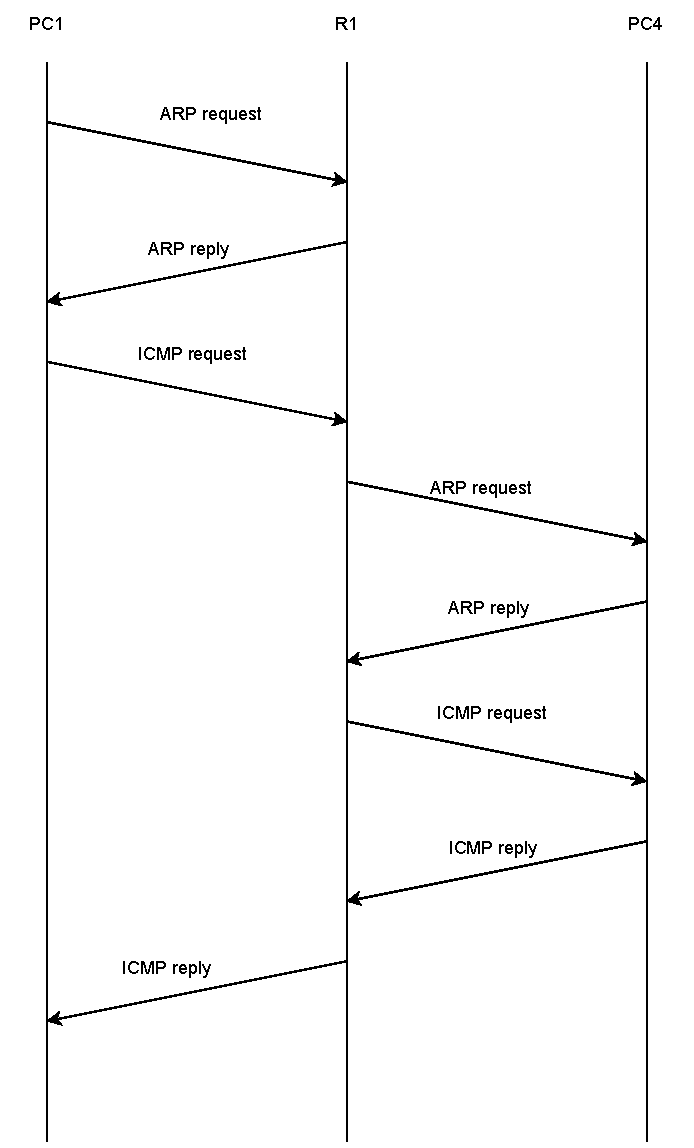
\includegraphics[width=0.5\linewidth]{\imagesPath/5.7.pdf}
		\end{figure}

	\subsection*{5.8}
		Καθαρίζουμε τους πίνακες ARP σε όλα τα μηχανήματα με \verb|arp -d -a|. Ξεκινάμε τις ζητούμενες καταγραφές στα PC3, PC4 και R1 για το LAN2, με τις εντολές:
		
		\begin{verbatim}
			PC3: tcpdump -e -i em0 "icmp or arp"
			PC4: tcpdump -e -i em0 "icmp or arp"
			R1: tcpdump -e -i em1 "icmp or arp"
		\end{verbatim}

	\subsection*{5.9}
		Από νέο παράθυρο στο PC3 κάνουμε ping στο PC4 με την εντολή \verb|ping -c 1 192.168.1.29|. Το ping είναι επιτυχές. Επίσης, στην έξοδο του ping παρατηρούμε ότι ελήφθη ένα μήνυμα ICMP redirect (New addr: 192.168.1.29) από τον R1.

	\subsection*{5.10}
		Σταματάμε τις καταγραφές και καταγράφουμε το περιεχόμενο των πινάκων ARP στα R1, PC3, PC4 (\verb|arp -a|):
		
		\begin{verbatim}
			PC3
			192.168.1.17 at 08:00:27:8b:5b:ee on em0 --> R1@em1
			192.168.1.18 at 08:00:27:a3:d0:ee on em0 --> PC3
			
			PC4
			192.168.1.29 at 08:00:27:fe:70:e0 on em0 --> PC4
			192.168.1.17 at 08:00:27:8b:5b:ee on em0 --> R1@em1
			192.168.1.18 at 08:00:27:a3:d0:ee on em0 --> PC3
			
			R1
			192.168.1.29 at 08:00:27:fe:70:e0 on em1 --> PC4
			192.168.1.17 at 08:00:27:8b:5b:ee on em1 --> R1@em1
			192.168.1.18 at 08:00:27:a3:d0:ee on em1 --> PC3
			192.168.1.14 at 08:00:27:40:c2:01 on em0 --> R1@em0
		\end{verbatim}

	\subsection*{5.11}
		\begin{figure}[H]
			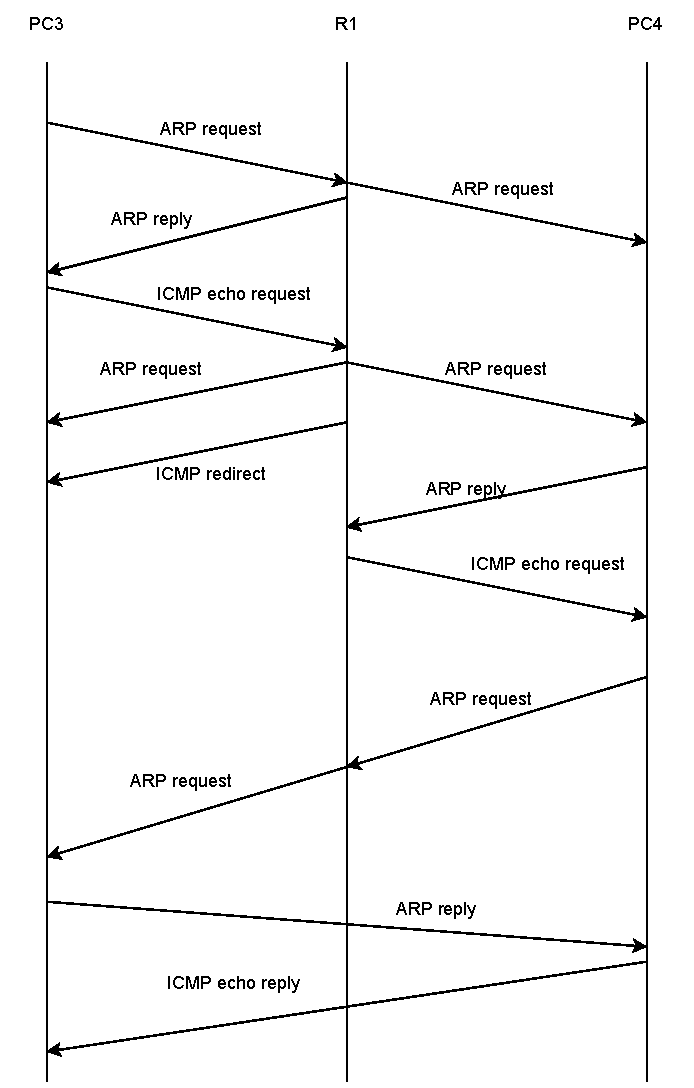
\includegraphics[width=0.75\linewidth]{\imagesPath/5.11.pdf}
		\end{figure}

	\subsection*{5.12}
		To PC3 αναζητεί με ARP τη διεύθυνση του R1@em1, ενώ το PC4 αναζητεί τη διεύθυνση του PC3.

	\subsection*{5.13}
		Το μήνυμα ICMP request του PC3 αποστέλλεται προς τον R1 και όχι απευθείας στον PC4 διότι ο PC3 βλέπει πως ο PC4 βρίσκεται σε διαφορετικό υποδίκτυο, οπότε στέλνει το μήνυμα στην προεπιλεγμένη πύλη, δηλαδή στον R1.

	\subsection*{5.14}
		Ο R1 χειρίζεται το προηγούμενο ICMP request στέλνοντας ένα μήνυμα ICMP redirect στον PC3, ώστε να τον ενημερώσει ότι το επόμενο σωστό βήμα ήταν ο PC4 και όχι ο R1. 

	\subsection*{5.15}
		Η απάντηση ICMP reply του PC4 στο PC3 στάλθηκε απευθείας.

	\subsection*{5.16}
		Εκτελούμε: 
		
		\begin{verbatim}
			PC3: tcpdump -e -i em0 "icmp"
			PC4: tcpdump -e -i em0 "icmp"
			R1: tcpdump -e -i em1 "icmp"
		\end{verbatim}

	\subsection*{5.17}
		Κάνουμε \verb|ping 192.168.1.29| από το PC3 στο PC4. Παρατηρούμε ότι ο PC3 λαμβάνει συνεχώς ICMP redirect από τον R1, ο οποίος προσπαθεί να τον ενημερώσει ότι το επόμενο σωστό βήμα δεν είναι ο R1 αλλά το PC4. Κατά τα άλλα η σχετική με το ping κίνηση κυκλοφορεί κανονικά. (ο R1 προωθεί το ICMP echo request στον PC4, και ο PC4 απαντά, στέλνοντας απευθείας στον PC3 ICMP echo reply).

	\subsection*{5.18}
		Στο PC3 εκτελούμε \verb|ifconfig em0 192.168.1.18/28|. Η προκαθορισμένη διαδρομή (\verb|netstat -rn|) διαγράφεται από τον πίνακα δρομολόγησης, όπως ήταν αναμενόμενο.

	\subsection*{5.19}
		Στο PC3, εκτελούμε \verb|route add 192.168.1.24/29 192.168.1.17|. Ύστερα με την εντολή \verb|netstat -rn| βλέπουμε ότι ο πίνακας δρομολόγησης του PC3 για προορισμούς σε υποδίκτυα του \verb|192.168.0.0/16| είναι:
		
		\begin{verbatim}
			Destination        Gateway         Flags   Netif     Expire
			192.168.1.16/28    link#1          U       em0
			192.168.1.18       link#1          UHS     lo0
			192.168.1.24/29    192.168.1.17    UGS     em0
		\end{verbatim}

	\subsection*{5.20}
		Επαναλαμβάνουμε τις ζητούμενες καταγραφές στο LAN2:
		
		\begin{verbatim}
			PC3: tcpdump -e -i em0 "icmp"
			PC4: tcpdump -e -i em0 "icmp"
			R1: tcpdump -e -i em1 "icmp"
		\end{verbatim}
		
		Εκτελούμε πάλι \verb|ping 192.168.1.29|. Αυτή τη φορά το PC3 λαμβάνει μόνο μία φορά το μήνυμα ICMP redirect, επειδή πλέον επιλέγει το PC4 σαν επόμενο βήμα, όπως το συμβουλεύει ο R1, αφού PC3 και PC4 βρίσκονται στο ίδιο υποδίκτυο πλέον. Έτσι, μετά την αποστολή του ICMP redirect, ο R1 δεν εμπλέκεται πλέον στην επικοινωνία των PC3 και PC4 (αυτά επικοινωνούν μεταξύ τους απευθείας πλέον).

	\subsection*{5.21}
		Πλέον έχει προστεθεί στον πίνακα δρομολόγησης του PC3 η εγγραφή: 
		
		\begin{verbatim}
			Destination    Gateway        Flags   Netif    Expire
			192.168.1.29   192.168.1.29   UGHD    em0
		\end{verbatim}
		
		με τη βασική διαφορά ότι πρόκειται για εγγραφή με διεύθυνση προθέματος 32 bits, και άρα μεγαλύτερη προτεραιότητα.
		
	\subsection*{5.22} 
		To PC3 δεν επικοινωνεί με τα μηχανήματα του LAN1, διότι δεν υπάρχει καμία εγγραφή στον πίνακα δρομολόγησης που να αφορά τα μηχανήματα του LAN1, και δεν υπάρχει ούτε default gateway.
	
	\subsection*{5.23} 
		Ορίζουμε ως προεπιλεγμένη πύλη τον R1 με την εντολή \verb|route add default 192.168.1.17|. Η διαδρομή που θα επιλεχθεί αν κάνουμε ping από το PC3 στο PC4 είναι η απευθείας διαδρομή, διότι ο PC3 έχει λάβει υπόψιν του το ICMP redirect και έχει προσθέσει την κατάλληλη εγγραφή στον πίνακα δρομολόγησης του.
		
\section*{Άσκηση 6: Router on a stick}

	\subsection*{6.1}
		Στο R1, αλλάζουμε το Promiscuous mode σε "Allow VMs", και ύστερα με τις εντολές:
		
		\begin{verbatim}
			ifconfig bridge0 create
			ifconfig bridge0 addm em0 addm em1 up
		\end{verbatim}
		
		δημιουργούμε τη ζητούμενη γέφυρα.

	\subsection*{6.2}
		Στο PC1, δημιουργούμε τις ζητούμενες διεπαφές με τις εντολές:
		
		\begin{verbatim}
			ifconfig em0.5 create vlan 5 vlandev em0 inet 192.168.5.1/24
			ifconfig em0.6 create vlan 6 vlandev em0 inet 192.168.6.1/24
		\end{verbatim}

	\subsection*{6.3}
		Αντίστοιχα, στο PC2:
		
		\begin{verbatim}
			ifconfig em0.5 create vlan 5 vlandev em0 inet 192.168.5.2/24
		\end{verbatim}

	\subsection*{6.4}
		Αντίστοιχα, στο PC3:
		
		\begin{verbatim}
			ifconfig em0.6 create vlan 6 vlandev em0 inet 192.168.6.18/24
		\end{verbatim}
		
	\subsection*{6.5}
		Αντίστοιχα, στο PC4:
		
		\begin{verbatim}
			ifconfig em0.5 create vlan 5 vlandev em0 inet 192.168.5.29/24
		\end{verbatim}

	\subsection*{6.6}
		Από το PC3:
		\verb|ping 192.168.1.1| $\rightarrow$ επιτυχές \\
		\verb|ping 192.168.5.1| $\rightarrow$ ανεπιτυχές \\
		\verb|ping 192.168.6.1| $\rightarrow$ επιτυχές \\

	\subsection*{6.7}
		Από το PC4:
		\verb|ping 192.168.1.1| $\rightarrow$ επιτυχές \\
		\verb|ping 192.168.5.1| $\rightarrow$ επιτυχές \\
		\verb|ping 192.168.6.1| $\rightarrow$ ανεπιτυχές \\


	\subsection*{6.8} 
		Κάποια από τα ping απέτυχαν, διότι το PC3 δεν έχει εγγραφή στον πίνακα προώθησης σχετική με τη διεύθυνση \verb|192.168.5.1|, ενώ το PC4 δεν έχει εγγραφή στον πίνακα προώθησης σχετική με τη διεύθυνση \verb|192.168.6.1|.

	\subsection*{6.9} 
		Στο PC3 ορίζουμε ως νέα προεπιλεγμένη πύλη το PC1 με την εντολή:
		
		\begin{verbatim}
			route change default 192.168.6.1
		\end{verbatim}
		
		Πλέον μπορούμε να κάνουμε ping σε όλες τις διεπαφές του PC1, αφού όταν κάνουμε \verb|ping 192.168.5.1| προτιμάται η default gateway και το πακέτο δρομολογείται σωστά.

	\subsection*{6.10}
		Ναι, μπορούμε να κάνουμε ping από το PC4 σε όλες τις διεπαφές του PC2.

	\subsection*{6.11}
		Όχι, δεν μπορούμε να κάνουμε ping από το PC3 σε καμία από τις διεπαφές του PC2.

	\subsection*{6.12}
		Με την εντολή \verb|sysctl net.inet.ip.forwarding=1| ενεργοποιούμε τη λειτουργία προώθησης πακέτων IPv4 στο PC1, και στο PC2 ορίζουμε ως νέα προεπιλεγμένη πύλη την \verb|192.168.1.1| με την εντολή \verb|route change default 192.168.1.1|.

	\subsection*{6.13}
		Ναι, τώρα τα ping από το PC3 προς τις διεπαφές του PC2 επιτυγχάνουν.

	\subsection*{6.14}
		Καταγράφουμε (\verb|ifconfig em0|) τις διευθύνσεις MAC των PC1,2,3:
		
		\begin{itemize}
			\item PC1 $\rightarrow$ \verb|08:00:27:02:3e:c4|
			\item PC2 $\rightarrow$ \verb|08:00:27:5f:02:9c|
			\item PC3 $\rightarrow$ \verb|08:00:27:a3:d0:ee|
		\end{itemize}
		
		Ύστερα, καθαρίζουμε τα ARP tables σε αυτά με την εντολή \verb|arp -d -a|.
	
	\subsection*{6.15}
		Ξεκινάμε τις ζητούμενες καταγραφές στα PC1,2,3 με τις εντολές:
		
		\begin{verbatim}
			PC1: tcpdump -e -i em0
			PC2: tcpdump -e -i em0
			PC3: tcpdump -e -i em0
		\end{verbatim}

	\subsection*{6.16}
		Ανοίγουμε νέο παράθυρο εντολών στο PC3 και εκτελούμε την εντολή \verb|ping -c 1 192.168.1.2|. Η ανταλλαγή των πακέτων έχει ως εξής:
		
		\begin{figure}[H]
			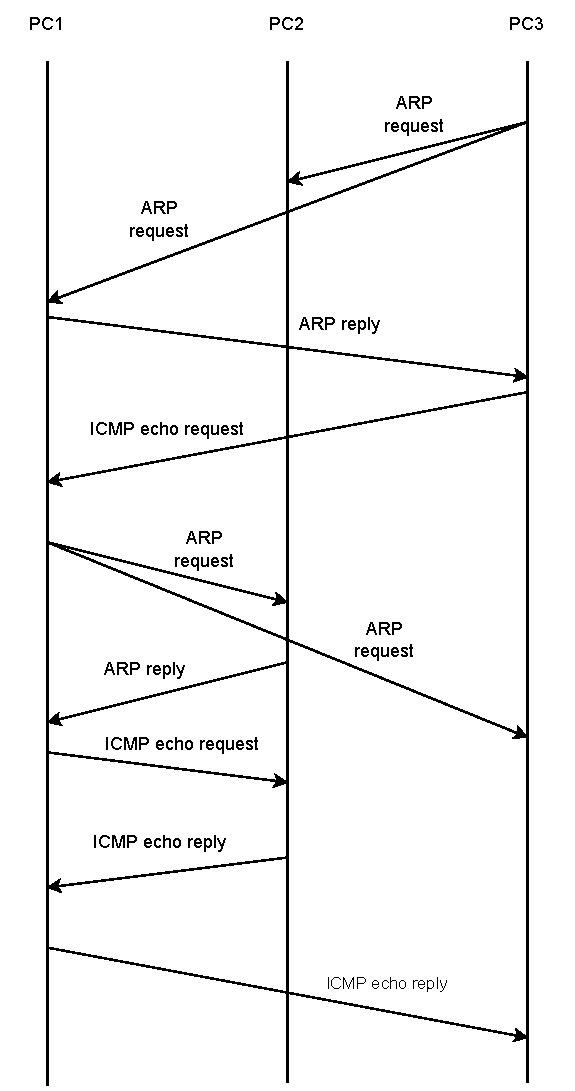
\includegraphics[width=0.65\linewidth]{\imagesPath/6.15.pdf}
		\end{figure}


	\subsection*{6.17}
		Ξεκινάμε ένα \verb|ping 192.168.5.29| από το PC3 προς τη διεπαφή του PC4 στο VLAN5 και το αφήνουμε να τρέχει. Το ping δεν είναι επιτυχές.

	\subsection*{6.18} 
		Ξεκινάμε τη ζητούμενη καταγραφή στο PC4 με την εντολή \verb|tcpdump -e -i em0|. Επιβεβαιώνουμε ότι ο PC4 δεν απαντά, παρόλο που λαμβάνει τα ICMP echo requests. Αυτό συμβαίνει επειδή το PC4 δεν έχει εγγραφή στον πίνακα δρομολόγησης που να αντιστοιχεί στη διεύθυνση από την οποία προέρχεται το ICMP echo request.

	\subsection*{6.19}
		Αλλάζουμε την προεπιλεγμένη πύλη με την εντολή \verb|route change default 192.168.5.1|. Τώρα το προηγούμενο ping επιτυγχάνει, αφού το PC4 προωθεί στην προεπιλεγμένη πύλη τα ICMP echo replies, και το PC1 αναλαμβάνει να τα προωθήσει στο PC3. 

\end{document}
